\apendice{Especificación de diseño}

\section{Introducción}
En este apartado se documentan los datos , la arquitectura, el procedimiento y la guía de estilo del proyecto.
\section{Diseño de datos}

El almacenamiento de datos se realiza en un fichero CSV denominado \texttt{webhook\_dataset.csv}, generado y mantenido por la aplicación Flask. Cada fila del fichero representa un conjunto de datos recibidos de TTN.

\begin{itemize}
    \item \textbf{timestamp (string)}: Fecha y hora ISO 8601 del mensaje.
    \item \textbf{occupied (boolean)}: Indica si se detectó movimiento.
    \item \textbf{button\_pressed (boolean)}: Estado del botón del sensor.
    \item \textbf{tamper\_detected (boolean)}: Detección de manipulación del sensor.
    \item \textbf{battery\_voltage (float)}: Voltaje actual de la batería (V).
    \item \textbf{temperature\_celsius (float)}: Temperatura medida (ºC).
    \item \textbf{humidity\_percent (float)}: Humedad relativa (\%).
    \item \textbf{time\_since\_last\_event\_min (int)}: Minutos desde el último evento.
    \item \textbf{event\_count (int)}: Contador de eventos.
    \item \textbf{tipo (string)}: Clasificación del dato (real o infectado).
\end{itemize}

Todos los datos son almacenados en texto plano, separados por comas y con codificación UTF-8.

\section{Diseño arquitectónico}


\section{Diseño procedimental}

A continuación se muestran distintos diagramas referentes a distintas acciones que se llevan a cabo durante el proyecto.

El primero es referente a la recepción y almacenamiento de datos:

\begin{figure}[H]
    \centering
    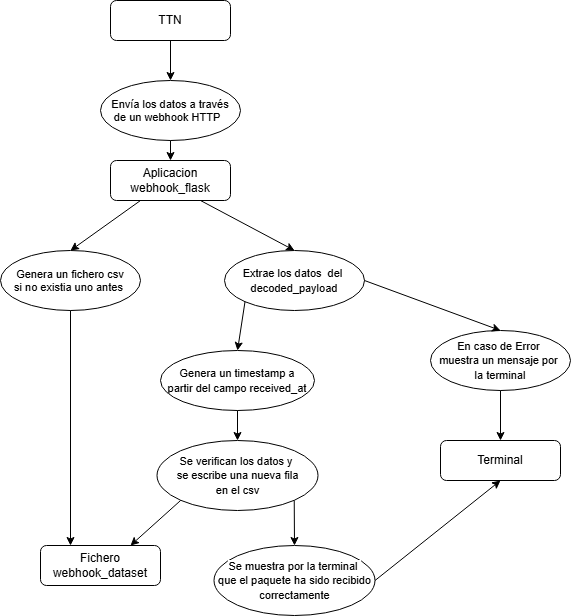
\includegraphics[width=0.8\linewidth]{img/diagrama_recep_alma}
    \caption{Diagrama de recepción y almacenamiento de datos.}
\end{figure}
Se va a representar otro diagrama referente a la visualización de los datos:

\begin{figure}[H]
    \centering
    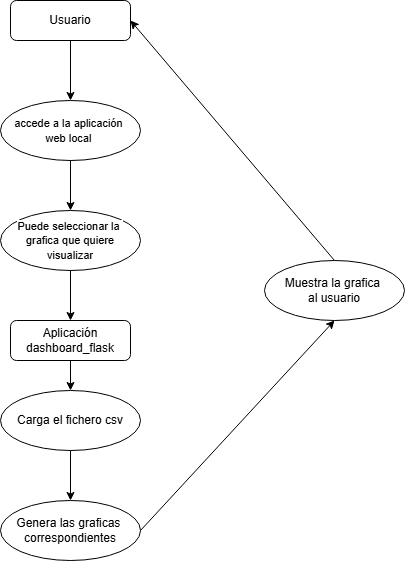
\includegraphics[width=0.6\linewidth]{img/diagrama_visual}
    \caption{Diagrama de visualización de la página web.}
\end{figure}

